{\textbf{1. 树的遍历}}{}

{树的遍历有两种方式:先根遍历和后根遍历。}

{{先根遍历}是先访问根结点,再依次访问根结点的每棵子树,访问子树时仍遵循先根再子树的规则。比如下图中的树进行先根遍历为:abeklfcgdhmij。}{}

{{后根遍历}是先依次访问根结点的每棵子树,再访问根结点,访问子树时仍遵循先子树再根的规则。比如下图中的树进行后根遍历为:klefbgcmhijda。}{}

{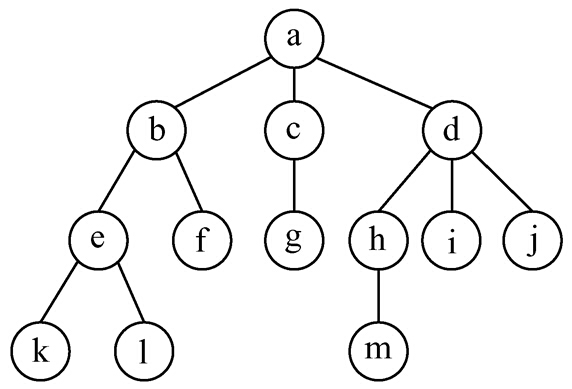
\includegraphics[width=2.08333in,height=2.08333in]{png-jpeg-pics/37d56eb30a4029dd9d455d19b9f4b080?}}

{\textbf{2. 森林的遍历}}

{森林的遍历有两种方式:先序遍历和后序遍历。}

{先序遍历森林}

{~ ~ ~ 若森林非空,则按下述规则遍历:}

{~ ~ ~~1)访问森林中第一棵树的根结点。}

{~ ~ ~ 2)先序遍历第一棵树中根结点的子树森林。}

{~ ~ ~ 3)先序遍历除去第一棵树之后剩余的树构成的森林。}

{~ ~ ~ 比如下图中的森林,先序遍历为:ABCDEFGHIJ。}

{中序遍历森林}

{~ ~ ~~若森林非空,则按下述规则遍历:}

{~ ~ ~ 1)中序遍历森林中第一棵树的根结点的子树森林。}

{~ ~ ~ 2)访问第一棵树的根结点。}

{~ ~ ~ 3)中序遍历除去第一棵树之后剩余的树构成的森林。}

{~ ~ ~ 比如下图中的森林,中序遍历为:BCDAFEHJIG。}

{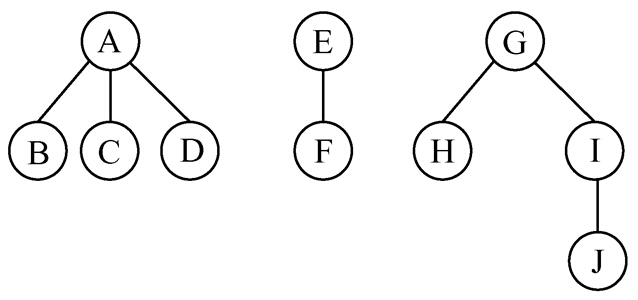
\includegraphics[width=2.08333in,height=2.08333in]{png-jpeg-pics/2a35ee42c99c72c88bb6a823cadca23d?}}
